% ==============================================================================
% SEÇÃO 3: PRÁTICA REDIS DIRETO NO BANCO (SEM PYTHON)
% ==============================================================================
\changecolours{ScoutRed}
\section{Redis Direto no Banco: CLI \& Redis Insight}

\begin{frame}{As 5 Estruturas de Dados Fundamentais do Redis}
  \centering
  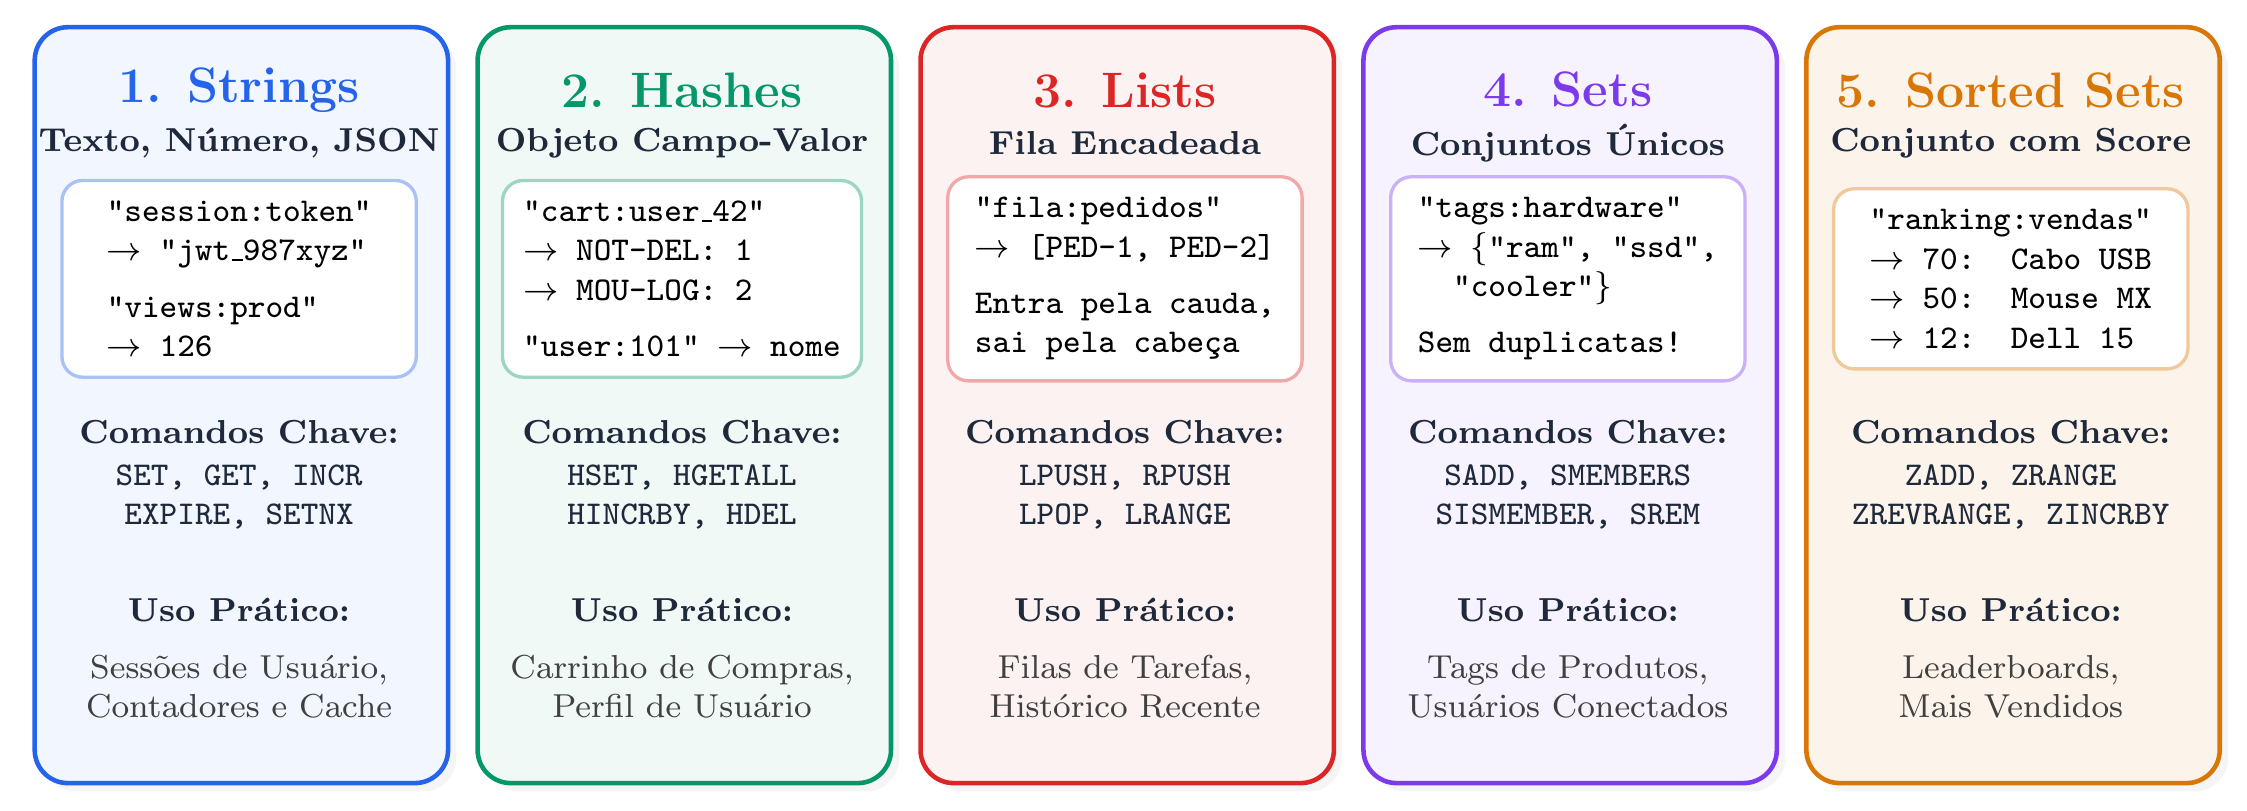
\includegraphics[width=0.98\textwidth,height=0.82\textheight,keepaspectratio]{figuras/fig_redis_estruturas.png}
\end{frame}

\begin{frame}{Operando com Redis Insight (Interface Gráfica)}
  \begin{columns}[T]
    \begin{column}{0.54\textwidth}
      \textbf{Recursos Visuais do Redis Insight}
      {\footnotesize
      \begin{enumerate}
        \item \textbf{Key Tree:} organiza chaves hierárquicas separadas por \texttt{:}.
        \item \textbf{Editor Visual:} inspeciona e edita Hashes, Listas e Sets em tempo real.
        \item \textbf{Memory Profiler:} analisa consumo de memória RAM por padrão de chave.
        \item \textbf{CLI Embutido:} terminal interativo acessível no rodapé.
      \end{enumerate}
      }
    \end{column}

    \begin{column}{0.44\textwidth}
      \begin{block}{Padrão de Nomes de Chaves}
        {\footnotesize
        Convenções recomendadas:
        \begin{itemize}
          \item \texttt{entidade:id}\\[1pt]
            {\scriptsize Ex: \texttt{user:101}}
          \item \texttt{entidade:id:subtipo}\\[1pt]
            {\scriptsize Ex: \texttt{cart:user:42}}
          \item \texttt{servico:escopo:chave}\\[1pt]
            {\scriptsize Ex: \texttt{cache:prod:01}}
        \end{itemize}
        }
      \end{block}
    \end{column}
  \end{columns}
\end{frame}

\begin{frame}[fragile]{Terminal redis-cli: Strings, TTL e Contadores}
  \textbf{Operações Chave-Valor Básicas e Expiração Automática:}
\begin{lstlisting}[basicstyle=\ttfamily\scriptsize]
// 1. Sessao temporaria com TTL de 120s
SET session:ads_user_42 "token_jwt_987" EX 120
GET session:ads_user_42       // Retorna o valor
TTL session:ads_user_42       // Retorna segundos restantes

// 2. Contador atomico de acessos
INCR views:produto:NOT-DEL-01
INCRBY views:produto:NOT-DEL-01 25

// 3. Trava distribuida atomica (Lock idempotente)
SET lock:pedido:9001 "worker_1" NX EX 30
\end{lstlisting}
\end{frame}

\begin{frame}[fragile]{Terminal redis-cli: Hashes e Carrinho de Compras}
  \textbf{Modelagem de Objetos e Carrinhos com Hashes:}
\begin{lstlisting}[basicstyle=\ttfamily\scriptsize]
// 1. Criar entidade com multiplos campos
HSET user:101 nome "Reginaldo Fernandes" campus "Taua" nivel "Docente"

// 2. Consultar campo individual e o hash completo
HGET user:101 nome
HGETALL user:101

// 3. Modelagem de Carrinho de Compras (SKU -> Quantidade)
HSET cart:session_taua_77 "NOT-DEL-01" 1 "MOU-LOG-02" 2

// 4. Incrementar item de forma atomica
HINCRBY cart:session_taua_77 "MOU-LOG-02" 1
\end{lstlisting}
\end{frame}

\begin{frame}[fragile]{Terminal redis-cli: Listas, Conjuntos e Rankings}
  \begin{columns}[T]
    \begin{column}{0.50\textwidth}
      \textbf{Filas FIFO com Lists}
\begin{lstlisting}[basicstyle=\ttfamily\tiny]
// Produtor enfileira na cauda
RPUSH fila:pedidos "PED-1" "PED-2"

// Consumidor retira da cabeca
LPOP fila:pedidos

// Consultar fila sem remover
LRANGE fila:pedidos 0 -1
\end{lstlisting}
    \end{column}

    \begin{column}{0.50\textwidth}
      \textbf{Rankings com Sorted Sets}
\begin{lstlisting}[basicstyle=\ttfamily\tiny]
// Adicionar score de vendas
ZADD ranking 45 "MOU-LOG-02"
ZADD ranking 12 "NOT-DEL-01"
ZADD ranking 70 "CAB-USBC-05"

// Top 3 mais vendidos (decrescente)
ZREVRANGE ranking 0 2 WITHSCORES
\end{lstlisting}
    \end{column}
  \end{columns}
\end{frame}
